%\section{Constraint space analysis}

%Constraints typisk bare på end effector på manipulatorer. Hvis de har constraints flere steder derimot som en slange har slangen en fordel at den kan komme seg "ut" fra flere vinkler --> end effector workspace er mye større når den kan utilize alt i verden til å dytte seg hit og dit og den kan krølle sammen halen.

%Constraint Jacobian vs task Jacobian.


\section{Task analysis}

Even though the control solution presented in \ref{subsec:DHPFC} decomposes the workspace in force and movement directions, there are some restrictions as to which tasks can be performed by the robot. To analyze this, it is beneficial to look at what kind of tasks a snake robot is required to achieve. In particular, the tasks of a snake robot moving according to the OAL principle will be covered in this section. Both a higher level path following goal and a lower level control goal is presented. It is the lower level goal that will be further researched in this project, but it is still important to keep in mind what the final purpose of the snake robot is.

Lastly, the task restrictions are discussed, followed by a mathematical adaption of the control scheme in \ref{subsec:DHPFC} based on the theory of West and Asada \cite{west1985method} described in \ref{subseq:HPFC}. This adaption is constructed to allow for the control of the task-relevant variables in cases where all task space variables can not be controlled independently.

\subsection{The overall task of the snake robot}

The motivation behind implementing the OAL principle on a snake robot is to make it move from one point in space to another by utilizing the obstacles present in its environment. In a "real world" situation, solely moving around is not enough and the snake robot will normally have some auxiliary assignment as well. This can typically be documenting its surroundings with a camera or similar equipment attached to its foremost link, referred to as its head. This again makes the snake robots exact path from the starting point to the end point relevant, and the path following of the head of the snake robot is thus the overall goal. When a path has been designed, this goal can be decomposed in tasks consisting of the global position and orientation of the snake robot head. In traditional robot manipulator theory, this would be referred to as the end-effector movement. 


\subsection{Lower level control tasks}

Because the base of traditional manipulators are fixed to the ground, they can move the end effector in a desired manner simply by following the inverse kinematics. This is of course given that the robots degrees of freedom satisfy the desired end effector movement. For snake robots, on the other hand, it is more complicated.
In order to reach the higher level path following goal, the snake robot has to push itself forward in a purposeful manner utilizing the obstacles in the environment. By purposeful it is here meant that the direction of the force application against the obstacles have to conform with the desired propulsion direction given by the path. This is where the hybrid position force control comes into play. The robot has to both position itself in a certain manner alongside the obstacles and push against them with a given force magnitude.

The general idea is that at any point in time a task will be given by a higher level path following algorithm which is assumed implemented. The information provided should include which obstacles are to be utilized and how the snake robot is to utilize them. In other words, the tasks sent to the hybrid position/force controller simply consist of a desired positioning (orientation) by every obstacle and force to be applied to the obstacles.



\subsection{Task restrictions}\label{subsec:task-restrictions}

The question that now arises is what the restrictions are to which tasks the higher level path following algorithm can command the snake robot to perform. It is obvious that not any given combination of position and force can be simultaneously achieved.

The restrictions lie in the composition of the snake robot, meaning how many joints the robot consists of. A higher number of joints, and thus actuators, enables the robot to control a higher number of variables. At the same time, a higher number of contact points impose a higher number of constraints on the system and therefore limit the controllability. That is not to say that few contact points are desired, because they are after all a necessity for successful propulsion.

For every contact point there are three possible variables that can be controlled. In \ref{subsec:DHPFC} it is defined that two of these variables belong to the position control. That is the movement along the obstacle and rotation by or around the obstacle. The remaining variable is reserved for the force against the obstacle.

To analyze the restriction to how many and which of these variables can be controlled for a given robot it is useful to look at the robots closed kinematic chains (CKCs). A kinematic chain is said to be closed when it contains one or more loops \cite{lynch2017modern}. In the snake robot case loops arise between points fixed in the world (base frame). That is the base of the robot, meaning the start of the first virtual translational joint, and every obstacle contact point. This is always true since it is assumed that the position of the obstacles are fixed in the world.

The number of CKCs is the same as the number of contact points on the robot. However, they can be expressed in several different ways. The first method is to define all closed kinematic chains from the base to every contact point. This is depicted in Figure \ref{fig:CKC1}, where $b$ denotes the base and $r_{c,i}$ denotes the different contact points.

\begin{figure}
    \centering
    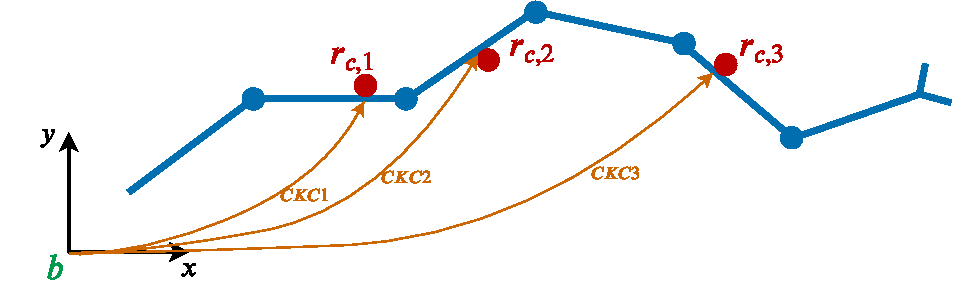
\includegraphics[width=0.9\textwidth]{figures/theory/CKC1.pdf}
    \caption{First method of defining the closed kinematic chains}
    \label{fig:CKC1}
\end{figure}

It is also possible to define the CKCs sequentially through the robot. Starting at the base again, the first CKC will be from the base to the first contact point. Moving further, the second chain will be from the first to the second contact point, then from the second to the third, etc. This definition of the CKCs is depicted in Figure \ref{fig:CKC2}, and will from now on be referred to as a minimal CKC representation. There are still many possible ways of defining the CKCs, but the two mentioned methods are the most relevant in this case.

\begin{figure}
    \centering
    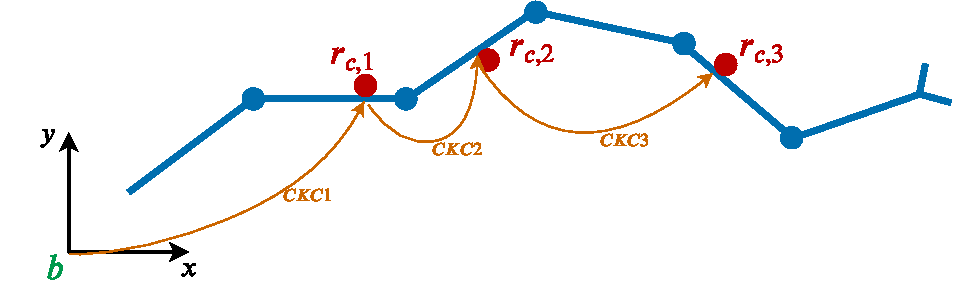
\includegraphics[width=0.9\textwidth]{figures/theory/CKC2.pdf}
    \caption{Second method of defining the closed kinematic chains}
    \label{fig:CKC2}
\end{figure}

The number of available actuators for controlling the variables at a single contact point are limited by the placement of the preceding contact point. This is because the CKC between these two points always is the smallest CKC with the least number of actuators and thus the so called bottleneck for the control.

To better explain this, an example snake robot is illustrated in figures \ref{fig:CKC1} and \ref{fig:CKC2}. In Figure \ref{fig:CKC1} there are four actuators included in the third CKC (CKC3) which is describing the third contact point. However, when looking at the closed kinematic chain for the same contact point described from its preceding contact point (depicted in Figure \ref{fig:CKC2}), only two actuators are included. Simply by studying the two figures it is also possible to see that the latter method always gives the minimal CKCs.

The ideal way of designing snake robots that require a high level of controllability is to include a very high number of joints. This way, even the minimal CKCs will have a sufficiently high number of actuators to make control at every contact point practically independent of the other contact points. Manipulators with such a large number of actuators are referred to as \textit{hyperredundant manipulators}. According to \cite{chiaverini2008kinematically}, a manipulator is considered to be hyperredundant if its controllable configuration space degrees of freedom are comparable to, or exceed, its task space degrees of freedom. Furthermore, it is stated that such manupulators have an enhanced potential to use their extra joints for maneuvering within tight obstacle fields. The term hyperredundant can be adopted to snake robots as well, and it is now obvious that hyperredundancy is a requirement for an ideal OAL-driven snake robot.

\subsubsection{Singularity avoidance}

A common problem when using Jacobian matrices for the inverse kinematic computations is the presence of singularities. A robot configuration $\mathbf{q}$ is singular if the task Jacobian matrix $\mathbf{J}_t$ is rank-deficient here \cite{chiaverini2008kinematically}. This configuration is not ideal since it means that it is impossible to generate task space velocities in certain directions. By task space velocities it is here meant velocity of the contact points vector $\mathbf{r}_t$, which is referred to as the end effector velocity in traditional robot manipulator theory.

An effect of a singularity is that the resulting joint space velocities can grow uncontrollably big. This effect is experienced not only at the singular configuration itself but also in its neighborhood \cite{chiaverini2008kinematically}. According to Chiaverini et al. \cite{chiaverini2008kinematically}, the distance to these singularities can be characterized through measurements based on the determinant of the Jacobian or the individual singular values of the matrix like the smallest singular value. If the snake robot consists of more joints than it needs for execution of the desired task, the additional degrees of freedom can be used to steer the snake robot away from singularities or avoid them at a planner level by analyzing these measurements. See \cite{chiaverini2008kinematically} for a more detailed description of the matter.
It should be noted that whether or not the robot is redundant depends both on the number of joints \textit{and} the number of contact points desired to control, i.e. the task.

Furthermore, the snake robot does not necessarily lose mobility in all task directions even though it is at a singular configuration. This is noteworthy since it might not be desirable for the snake robot to move in every possible direction anyway. In \ref{subsec:task-oriented} it is explained how the desirable or essential movement directions can be expressed and further utilized for control.


\subsection{Task oriented control scheme}\label{subsec:task-oriented}


\ref{subseq:HPFC} states that there are certain directions of force and movement that are essential for performing a task. It is further claimed that the number of essential directions can not be greater than the number of controllable actuators in the robot necessary for performing the task. \ref{subsec:task-restrictions} explained that the number of available controllable actuators is limited by the minimal CKC.

For the snake robot, the force and movement directions of a task are described by $\mathbf{E}_F$ and $\mathbf{E}_P$.
%In some cases, the number of directions described by these vectors might exceed the number of active joints even though not all directions \textit{have} to be controlled precisely in order to perform the given task. So in other words, t
The number of essential directions in $\mathbf{E}_F$ and $\mathbf{E}_P$ together can not exceed the number of active joints in the minimal CKC. In the example in Figure \ref{fig:CKC2}, a maximum number of three variables at the second contact point could be desired to control. However, it is seen that the corresponding CKC only contains one actuator, meaning that at most one variable has to be chosen for control. In other words, the maximum number of essential variables that can be defined for performing a task at the second contact point is one.

As explained in \ref{subseq:HPFC}, the essential position and force directions can be described by (\ref{eq:hpfc_wep}) and (\ref{eq:hpfc_wef}). The filters (\ref{eq:hpfc_fp}) and (\ref{eq:hpfc_ff}) can then be used to focus the control on these essential directions, also taking into account which directions the robot is allowed to move and apply force in. This is of course given that the requirements regarding the number of active joints are fulfilled.

The force filter $\prescript{}{j}{\mathbf{F}}_{f}$, which is based on the allowable and essential force directions, can intuitively be combined with the input torque $\boldsymbol{\tau}_F$ for the desired force found by (\ref{eq:dhpfc_tauf}). It should be noted that the defined essential force directions and desired forces $\mathbf{f}_{F,d}$ have to correspond with each other. Combining the position filter $\prescript{}{j}{\mathbf{F}}_{p}$ with the position control torque from (\ref{eq:dhpfc_taup}) is unfortunately not as intuitive. This is because the filter is designed to map the joint velocities and not joint torques. The DHPFC control structure simply takes the desired contact point variables and directly computes the desired joint accelerations. This means that there is no intermediate step with joint velocities, as would have been convenient for the position filtering.

Under certain conditions and requirements, however, there are ways of combining the filter directly with the position control torque $\boldsymbol{\tau}_P$. First of all, it is known that as long as the position control is in fact performed in the position space, any acceleration $\ddot{\mathbf{q}}$ should lead to a change in velocity rather than force application. This again means there is a direct relationship between the joint accelerations and the velocities leading to the same "rules" being applicable for the two variables. Second of all, it is known that at very low velocities, the relationship between the joint torques and joint accelerations become approximately linear. This is because the moment of inertia of the links is constant in the used snake robot model. Again, it can be stated that the same rules apply for the position torque and desired position joint accelerations. Conclusively, the position filter $\prescript{}{j}{\mathbf{F}}_{p}$ can be used directly on the input torque for the desired position. It is again important that the essential position directions and desired position variables correspond.

Under the mentioned conditions, the new input control torques can be found by

\begin{equation}
    \boldsymbol{\tau}_c = \prescript{}{j}{\mathbf{F}}_{p} \boldsymbol{\tau}_P + \prescript{}{j}{\mathbf{F}}_{f} \boldsymbol{\tau}_F.
\end{equation}
